\documentclass[11pt]{article}

% Paper: plain article + pdflatex (arXiv TeX Live safe).
\usepackage[T1]{fontenc}
\usepackage{lmodern}
\usepackage[utf8]{inputenc}
\usepackage{amsmath,amssymb}
\usepackage{graphicx}
\usepackage{booktabs}
\usepackage{array}
\usepackage{tabularx}
\usepackage{longtable}
\usepackage[margin=1in]{geometry}
\usepackage{xcolor}
\usepackage{microtype}
% expansion=false is an arXiv-safety choice; protrusion must be off
% with it (protrusion-only interacts pathologically with long
% unbreakable tokens, producing large overfull boxes).
\microtypesetup{expansion=false,protrusion=false}
% Emergency-stretch safety net: keeps normal line-breaking, adds a
% third pass so tight paragraphs with long unbreakable tokens (file
% paths, identifiers) never produce overfull boxes.
\setlength{\emergencystretch}{2em}
\usepackage[section]{placeins}
\usepackage[numbers,sort&compress]{natbib}
\usepackage[colorlinks=true,linkcolor=blue!60!black,citecolor=blue!60!black,urlcolor=blue!60!black]{hyperref}
\hypersetup{
  pdftitle={Characterizing a Low-Dimensional Redshift-Dependent Difference Between CMB- and Distance-Compatible Expansion Histories},
  pdfauthor={Jake Enholm},
  pdfsubject={Redshift-dependent comparison of distance-sector and Planck-calibrated expansion histories}
}

% Numerical results are NEVER hand-copied into the manuscript.
% Every number below comes from paper/generated/results_macros.tex,
% generated by scripts/paper/build_results_registry.py from versioned
% machine-readable evidence.
% GENERATED FILE -- do not edit by hand.
% Owner: scripts/paper/build_results_registry.py
% Source of truth: paper/evidence/ (versioned publication evidence).
% Publication mode: neutral macros only.

\newcommand{\BridgeAIC}{1469.96}
\newcommand{\BridgeAICCtrl}{1493.92}
\newcommand{\BridgeAICDeltaVsCtrl}{-23.96}
\newcommand{\BridgeChiTwo}{1459.96}
\newcommand{\BridgeDeltaCtrl}{8.04}
\newcommand{\BridgeDesiBareConstr}{18.08}
\newcommand{\BridgeDesiMThreeConstr}{11.17}
\newcommand{\BridgeEpsDelta}{0.124}
\newcommand{\BridgeKCtrl}{21}
\newcommand{\BridgeKmThree}{5}
\newcommand{\BridgeNullDesiConstr}{-6.90}
\newcommand{\BridgeNullSn}{-76.1}
\newcommand{\BridgeRank}{5}
\newcommand{\CmbOneHZero}{67.99}
\newcommand{\CmbTwoHZero}{67.4}
\newcommand{\CvConstrBootProb}{0.216}
\newcommand{\CvConstrLyaProb}{0.788}
\newcommand{\CvConstrMFive}{8186.77}
\newcommand{\CvConstrMFour}{8164.15}
\newcommand{\CvConstrMSix}{8184.01}
\newcommand{\CvConstrMThree}{8164.28}
\newcommand{\CvConstrMTwo}{8213.92}
\newcommand{\CvConstrSelected}{3}
\newcommand{\DistanceHZero}{72.80}
\newcommand{\GeometryCmbRatioHigh}{0.013}
\newcommand{\GeometryCmbRatioLow}{0.037}
\newcommand{\GeometryCommonFractionMin}{0.998}
\newcommand{\GeometryCosineSimilarity}{0.9997}
\newcommand{\GeometryPeakZ}{0.65}
\newcommand{\GeometryPrincipalAngle}{1.5}
\newcommand{\GeometrySvdDominance}{76.3}
\newcommand{\GeometryTransferDegradation}{0.068}
\newcommand{\ReferenceSensitivityRatioMaxPct}{8.4}
\newcommand{\ReferenceSensitivityRatioMinPct}{1.3}


\newcommand{\kmsMpc}{\ensuremath{\,\mathrm{km\,s^{-1}\,Mpc^{-1}}}}

\title{%
  Characterizing a Low-Dimensional Redshift-Dependent Difference
  Between CMB- and Distance-Compatible Expansion Histories
}
\author{Jake Enholm}
\date{\today}

\begin{document}
\maketitle

\begin{abstract}
Under the endpoint constructions examined here, low-redshift distance data and Planck-calibrated references favor substantially different best-fit expansion histories: neither side fits the full DESI DR2, Pantheon+SH0ES, and
Planck TT/TE/EE likelihood contract at once, and none of the tested endpoints simultaneously supplies a complete fit to all sectors. We compare three fixed
endpoints over the constrained domain $z\le1.8$: a phenomenological
low-redshift distance-sector endpoint~R reaching
$H_{0}=\DistanceHZero$\kmsMpc{}, a
Planck-calibrated reference~C1 with
$H_{0}=\CmbOneHZero$\kmsMpc{}, and a secondary
Planck-compatible reference~C2 with $H_{0}=\CmbTwoHZero$\kmsMpc{}
(a separately implemented sensitivity check sharing the same Planck
sky, not an independent confirmation).
Within the predeclared reconstruction family, constrained-domain predictive
validation (SN plus DESI $z\le1.8$ folds; Ly$\alpha$ scored separately
as a failed continuation test) selects a
compact five-coordinate order-3 map of the endpoint difference with
local projected Jacobian rank~5 of~5 fitted coordinates
($\chi^{2}=\BridgeChiTwo{}$, only \BridgeDeltaCtrl{} above the
21-coordinate control).
The fixed order-3 map improves held-out supernova prediction by $\Delta\chi^{2}=\BridgeNullSn{}$
against the null reconstruction (the undeformed $\Lambda$CDM reference, with zero fitted reconstruction
coordinates and the common SN nuisance parameter profiled normally) and improves constrained DESI ($z\le1.8$) by
$\Delta\chi^{2}=\BridgeNullDesiConstr{}$ (null reconstruction $\chi^{2}=\BridgeDesiBareConstr{}$ against
$m=3$ $\chi^{2}=\BridgeDesiMThreeConstr{}$); the order-3 reconstruction fails its separate $z=2.33$ Ly$\alpha$ continuation test strongly, and the matched constrained-domain null
bootstrap (250 replicates; same null/candidate family, data split,
bounds and selection rule) gives
$P(\mathrm{select}\ge m{=}3)=\CvConstrBootProb{}$ with
Ly$\alpha$ continuation-failure fraction~\CvConstrLyaProb{} recorded separately.
Zero ruler-clock split is allowed
($\Delta\chi^{2}(\epsilon{=}0)=\BridgeEpsDelta{}$).
The reference-sensitivity check shows that the difference between R and C1 and the difference between R and C2 share one
dominant direction (cosine~\GeometryCosineSimilarity{},
principal angle~\GeometryPrincipalAngle$^{\circ}$,
common-mode fraction $\ge\GeometryCommonFractionMin{}$ per interval,
largest amplitude near $z\approx\GeometryPeakZ{}$). Across the constrained redshift bins, the RMS difference between C1 and C2 is approximately 1\% to 8\% of the corresponding RMS difference between R and either Planck reference.
In plain terms, the distance-sector endpoint has a systematically higher $H(z)$ than the Planck-calibrated references, and the size of that difference changes with redshift rather than behaving like a single constant $H_0$ offset. A five-coordinate order-3 reconstruction captures this redshift-dependent pattern over $z\le1.8$, with its largest endpoint separation near $z\approx0.65$; the separate Ly$\alpha$ continuation test at $z=2.33$ fails.

\end{abstract}

\section{Introduction}
\label{sec:intro}

The Hubble tension is an observational disagreement between the local
supernova distance ladder,
$H_{0} = 73.04 \pm 1.04$\kmsMpc{} \citep{Riess2022}, and the Planck
2018 TT/TE/EE spectrum, $67.4 \pm 0.5$\kmsMpc{} in flat $\Lambda$CDM
\citep{Planck2018}, reviewed in \citet{Verde2019} and
\citet{KnoxMillea2020}. The mismatch extends beyond a single number:
DESI DR2 BAO \citep{DESIDR2} sharpens the late-time
distance--redshift relation while the Pantheon+SH0ES compilation
\citep{Scolnic2022,Brout2022} maps the supernova expansion history,
and neither a distance-calibrated nor a CMB-calibrated history fits
all sectors at once. Observed values, uncertainties, and covariance
matrices are held fixed across model comparisons; only theory
predictions change between branches.

The standard question this paper asks is: is the disagreement
reducible to a compact redshift-dependent difference between
independently calibrated background histories? Rather than fitting
another cosmological model with additional dynamical freedom, we test
whether the observable gap between already-calibrated endpoints has
low-dimensional, predictable structure.

The experimental design uses three frozen endpoints. The
distance-compatible history~R reaches
$H_{0}=\DistanceHZero$\kmsMpc{} and fits DESI DR2 BAO and
Pantheon+SH0ES supernovae. The CMB-compatible history~C1 is a Planck TT/TE/EE-compatible
reference with $H_{0}=\CmbOneHZero$\kmsMpc{} produced with the stated
CAMB/likelihood configuration. The secondary Planck-compatible reference~C2 is a
separately implemented baseline with
$H_{0}=\CmbTwoHZero$\kmsMpc{}, built through its own likelihood and
spectral-parity path for reference-sensitivity checking. C1 and C2 are separately implemented in pipeline/model space, not statistically
independent in data space: they share the
Planck sky but differ in construction pipeline, parameter choices,
and calibration route.

This differs from fitting another cosmological model in four ways.
First, the endpoints are constructed separately, before any
comparison is made. Second, bridge dimensionality is selected with
held-out prediction, not training $\chi^{2}$. Third, higher
flexibility is allowed to fail: overfitting orders and
boundary-limited families are retained as frozen adversarial
controls. Fourth, the reference-branch robustness test changes the CMB
reference branch without changing the hypothesis: the same compact
map must describe both $\Delta_{1}$ and $\Delta_{2}$.

The headline result, over the constrained domain $z\le1.8$, is
\[
\Delta_{1}(z) \simeq \Delta_{2}(z),
\qquad
\|\Delta_{C}\| \ll \|\Delta_{1,2}\|,
\]
where the fields
$\Delta_{1}(z)\equiv\ln H_{R}(z)-\ln H_{C_{1}}(z)$,
$\Delta_{2}(z)\equiv\ln H_{R}(z)-\ln H_{C_{2}}(z)$, and
$\Delta_{C}(z)\equiv\ln H_{C_{1}}(z)-\ln H_{C_{2}}(z)$
are defined in Section~\ref{sec:endpoint-repr} and summarized in the
nomenclature table (Table~\ref{tab:nomenclature}).
The two R--CMB difference fields share one dominant direction
(cosine~\GeometryCosineSimilarity{}, principal angle
\GeometryPrincipalAngle$^{\circ}$), peak near
$z\approx\GeometryPeakZ{}$, and transfer across branches with
fractional residual degradation~\GeometryTransferDegradation{},
whereas the CMB--CMB difference is much smaller
throughout (about 1--8\% of the R--CMB difference across the
constrained bins).

In plain terms, the distance-sector endpoint requires a
systematically higher expansion rate than the Planck-calibrated
references, and the size of that mismatch changes with redshift
rather than behaving like a simple constant $H_{0}$ offset. A compact
five-parameter map summarizes that pattern over $z\le1.8$, but its
statistical significance and physical origin are not established, and
the same compact extrapolation fails at the Ly$\alpha$ point at
$z=2.33$.

This paper identifies and characterizes that empirical deformation.
The principal result of this work is therefore not a specific
dynamical model, but an empirically defined expansion-history target
that candidate explanations of the CMB--distance discrepancy can be
tested against. Its physical origin remains deliberately unaddressed.
Section~\ref{sec:endpoints} defines the data and the R, C1, and C2
endpoints (with the nomenclature table immediately below);
Section~\ref{sec:methods} the empirical reconstruction method;
Section~\ref{sec:bridge} the predictive model-selection tests;
Section~\ref{sec:robustness} the reference-branch robustness test;
Section~\ref{sec:results} the results;
and Sections~\ref{sec:discussion}--\ref{sec:conclusion} the
interpretation, limitations, and conclusions.

% Ch 2. Data and endpoint definitions (section heading in
% 02_endpoint_construction; 03 contributes subsections only).
\section{Data and endpoint definitions}
\label{sec:endpoints}
\label{sec:data-endpoints}

The three expansion histories compared in this paper were obtained
separately, before any comparison was made. Each is fixed: no
endpoint is refit, retuned, or extended anywhere in this analysis.
All headline values resolve through generated macros to the fixed
artifacts cited below. Symbols are defined once in the nomenclature
table (Table~\ref{tab:nomenclature}); throughout the main text,
R is the distance-compatible endpoint, C1 and C2 are the two
Planck-compatible endpoints, and the order-3 representation is the selected compact
reconstruction basis.

\begin{table}[!htbp]
  \centering
  \caption{Nomenclature: symbols used in the main analysis.}
  \label{tab:nomenclature}
  \begin{tabularx}{\linewidth}{lXXX}
    \toprule
    Symbol & Meaning & How obtained & Used for \\
    \midrule
    $R$ & distance-sector endpoint &
      fixed distance-sector endpoint & reference deformation \\
    $C_{1}$ & Planck-calibrated reference &
      Planck TT/TE/EE calibrated CAMB reference & CMB reference \\
    $C_{2}$ & secondary Planck-calibrated reference &
      separately implemented Planck/CAMB reference & sensitivity reference \\
    $\Delta_{1}$ & $\ln H_{R}(z)-\ln H_{C_{1}}(z)$ &
      derived & comparison \\
    $\Delta_{2}$ & $\ln H_{R}(z)-\ln H_{C_{2}}(z)$ &
      derived & comparison \\
    $\Delta_{C}$ & $\ln H_{C_{1}}(z)-\ln H_{C_{2}}(z)$ &
      derived & reference spread \\
    $K_{H}$ & overall amplitude of the reconstruction map &
      fitted (reconstruction coordinate) & compact representation \\
    $c_{j}$ & Legendre shape coefficients ($j=0,1,2$) &
      fitted (reconstruction coordinates) & compact representation \\
    $m=3$ & order-3 reconstruction &
      CV-selected & compact representation \\
    $\epsilon$ & reciprocity parameter &
      profiled & diagnostic only \\
    \bottomrule
  \end{tabularx}
\end{table}


\subsection{Distance-compatible endpoint R}
\label{sec:endpoint-r}

R is the fixed phenomenological distance-sector endpoint used in this comparison. It reaches $H_0=72.80$~km~s$^{-1}$~Mpc$^{-1}$, carries $r_d=135.39$~Mpc, and provides the low-redshift distance-sector reference history. The
compressed distance prior \citep{Chen2019} used during endpoint
discovery was validated only for conventional late-time models; it did
not validate the $r_{d}=135.39$~Mpc early-universe physics.

Concretely, R is the smooth low-redshift reference history
(pinned in
\path{paper/evidence/endpoints/endpoint_manifest.json}).
It reaches $H_{0}=\DistanceHZero$\kmsMpc{} with
$r_{d}=135.39$~Mpc and fits the DESI DR2 and Pantheon+SH0ES distance
sector. Nothing in Sections~\ref{sec:model-selection} or
\ref{sec:reference-sensitivity} depends on the history of how R was found.

\subsection{CMB-compatible endpoint C1}
\label{sec:endpoint-c1}

C1 is a Planck TT/TE/EE-compatible reference background with
$H_{0}=\CmbOneHZero$\kmsMpc{} and
$r_{\mathrm{drag}}=147.15$~Mpc, produced with the stated
CAMB/likelihood configuration.
No distance-sector parameter, table, or likelihood entered its construction.

\subsection{Secondary Planck-compatible reference C2}
\label{sec:endpoint-c2}

C2 is a secondary Planck-compatible $\Lambda$CDM reference with
$H_{0}=\CmbTwoHZero$\kmsMpc{}, used only as a reference-sensitivity
check, evaluated through its own Planck
likelihood. It shares the
Planck sky with C1 and uses nearly the same $\Lambda$CDM background
family with its own parameter choices and calibration route, so it
cannot provide independent cosmological confirmation. C1
and C2 are separately implemented in pipeline/model space, not
statistically independent in data space; both use Planck
information. Table~\ref{tab:endpoint-construction} compares the two
constructions row by row.

\subsection{Common observable representation}
\label{sec:endpoint-repr}

All three endpoints are compared on one common uniform-$u$ grid of
2000 nodes spanning $0 \le z \le 2.33$
(\path{paper/evidence/endpoints/endpoint_redshift.json}). The
difference fields
\[
\Delta_{1}(z) \equiv \ln H_{R}(z)-\ln H_{C_{1}}(z), \qquad
\Delta_{2}(z) \equiv \ln H_{R}(z)-\ln H_{C_{2}}(z), \qquad
\Delta_{C}(z) \equiv \ln H_{C_{1}}(z)-\ln H_{C_{2}}(z)
\]
are evaluated on that grid and fixed in
\path{paper/evidence/reference_sensitivity/difference_fields.npz}. The
constrained domain is $z \le 1.8$, covering all non-Ly$\alpha$ DESI
blocks; the Ly$\alpha$ anchor at $z=2.33$ tests the continuation law,
not the low-redshift deformation
(\path{paper/evidence/reference_sensitivity/domain_split.json}).

\begin{figure}[!htbp]
  \centering
  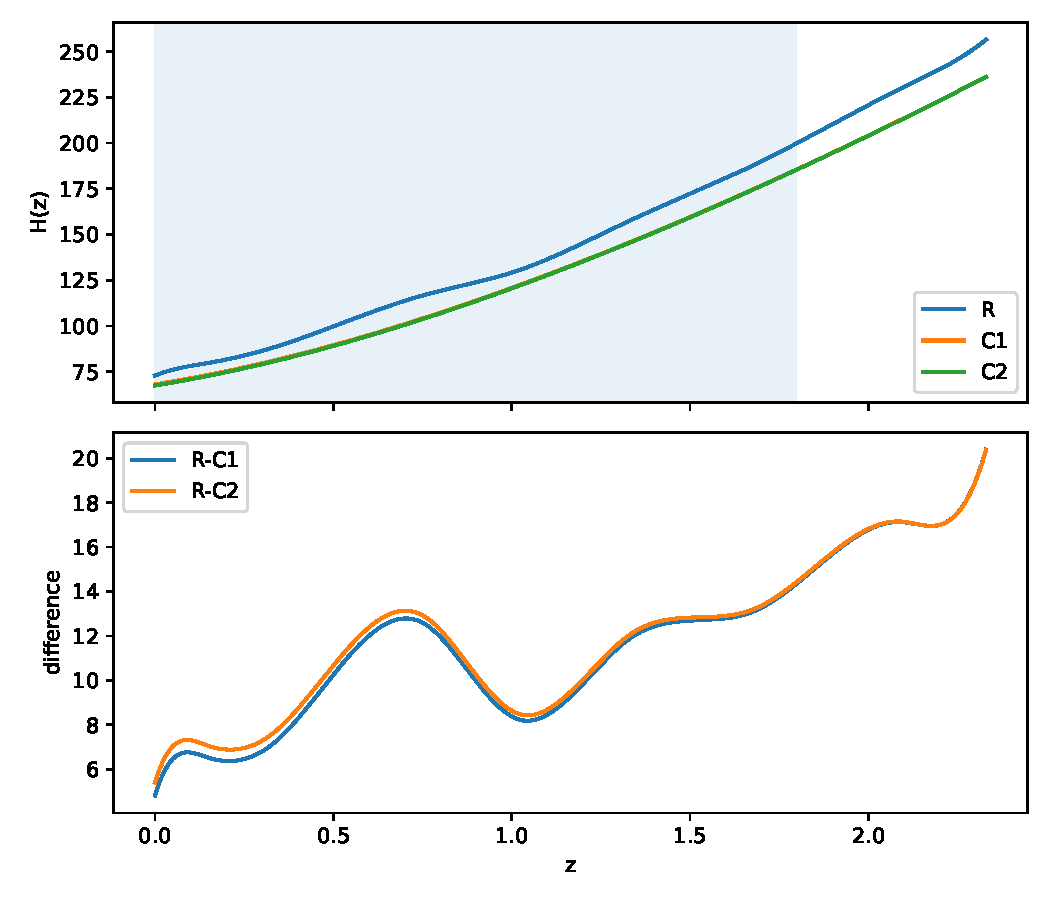
\includegraphics[width=0.9\linewidth]{figures/generated/overview_fig1_endpoints}
  \caption{Fixed endpoint overview (no fits in this figure). Top: the
  three fixed histories $H_{R},H_{C_{1}},H_{C_{2}}$; C1 and C2 nearly
  overlap in the upper panel and distinct line styles are used to keep
  both visible. Bottom: their
  logarithmic differences $\Delta_{1},\Delta_{2},\Delta_{C}$; across
  the constrained bins the RMS difference between C1 and C2 is approximately 1\% to 8\% of
  the corresponding RMS difference between R and either Planck reference.
  Shading marks the constrained domain $z\le1.8$; the dotted line
  marks the Ly$\alpha$ continuation test at $z=2.33$.}
  \label{fig:endpoint-overview}
\end{figure}

\subsection{Endpoint acoustic calibration}
\label{sec:calibration}

Each endpoint carries its own acoustic ruler, traced to fixed
artifacts in the endpoint calibration contract
(\path{paper/evidence/endpoints/calibration_contract.json}). Boltzmann
rulers are computed with CAMB \citep{Lewis2000}:

\begin{table}[!htbp]
  \centering
  \caption{Endpoint acoustic calibration: every endpoint's ruler.
  The compressed distance prior \citep{Chen2019} did not validate
  nonstandard early-universe physics for R.}
  \label{tab:calibration}
  \begin{tabular}{lllll}
    \toprule
    Endpoint & $r_{d}$ [Mpc] & $r_{s}$ [Mpc] &
      Fixed or recomputed? & Source \\
    \midrule
    R & 135.39 & --- (not used) &
      fixed (pinned control fit) & control fit \\
    C1 & 147.15 & 144.50 &
      recomputed (CAMB stage-0) & stage-0 background \\
    C2 & 147.11 & 144.45 &
      recomputed (CAMB baseline) & baseline acoustic \\
    \bottomrule
  \end{tabular}
\end{table}

R uses an early-ruler value different from C1/C2; this ruler
difference is part of the measured endpoint separation, not a shared
calibration. The R ruler is roughly $0.92$ of either CMB ruler, an
$\sim8\%$ smaller ruler. This is a property of the phenomenological
distance endpoint, not a demonstrated physical sound horizon: R's
$r_{d}=135.39$~Mpc is a phenomenological endpoint value and is not
validated as early-universe physics. The compressed Planck distance
prior \citep{Chen2019} was validated only for conventional
$\Lambda$CDM, $w$CDM, and CPL models and cannot by itself validate
such nonstandard pre-recombination physics; no BBN viability is
claimed (no BBN fit is performed). The BAO forward model is endpoint-specific:
\begin{equation}
  D_{M}/r_{d},\qquad D_{H}/r_{d},\qquad D_{V}/r_{d},
  \label{eq:bao-forward}
\end{equation}
evaluated with each endpoint's own ruler from
Table~\ref{tab:calibration}.

\begin{table}[!htbp]
  \centering
  \caption{Endpoint construction comparison: C1 versus C2.}
  \label{tab:endpoint-construction}
  {\small
  \begin{tabularx}{\linewidth}{lXX}
    \toprule
     & C1 & C2 \\
    \midrule
    Underlying CMB observations & Planck TT/TE/EE & Planck TT/TE/EE \\
    Boltzmann code & CAMB 2.0.4 & CAMB (baseline pipeline) \\
    Likelihood implementation & Planck TT/TE/EE likelihood (CAMB-based) &
      stock baseline Planck likelihood \\
    Cosmological parameterization & flat $\Lambda$CDM stage-0 &
      flat $\Lambda$CDM \\
    Primordial spectrum parameterization & power-law tilt &
      power-law tilt, $n_{s}=0.965$ \\
    Optimizer/sampler & background tuning (stage-0) &
      fixed-parameter baseline with spectral parity \\
    Background extraction & frozen CAMB table &
      CAMB-sampled $H(z)$ table \\
    $H_{0}$ [km\,s$^{-1}$\,Mpc$^{-1}$] & 67.99 & 67.4 \\
    $\Omega_{m}$ & 0.3075 & 0.3134 \\
    $r_{d}$ [Mpc] & 147.15 & 147.11 \\
    $r_{s}$ [Mpc] & 144.50 & 144.45 \\
    \bottomrule
  \end{tabularx}
  }
\end{table}

C1 and C2 are separately implemented in pipeline/model space,
not statistically independent in data space; both use Planck
information.


\label{sec:data}
% Part of Section~2 (Data and endpoint definitions): likelihood details.
% This file contributes subsections only; the section heading lives in
% 02_endpoint_construction.tex.

Observed values, uncertainties, and covariance matrices are held fixed
across model comparisons. Only theory
predictions change. What follows groups the likelihoods into the
low-redshift distance sector, the high-redshift CMB sector, and the
controls that keep the comparison honest.

\subsection{Low-redshift distances}

DESI DR2 BAO \citep{DESIDR2} enters through the collaboration
distance ratios $D_{M}/r_{d}$, $D_{H}/r_{d}$, $D_{V}/r_{d}$ with the
published covariances; DESI values are fixed and only the theory
prediction changes between branches.

The supernova block is the full Pantheon+SH0ES compilation
\citep{Scolnic2022,Brout2022,Riess2022} as one 1657-row covariance likelihood
with one common profiled absolute magnitude $M$ (row-selection contract,
\path{paper/evidence/sn_selection_contract.json}: 1701 raw rows
selected by the exact mask \texttt{(zHD > 0.01) | IS\_CALIBRATOR} to
1657 rows, of which 77 calibrators and 1580 Hubble-flow rows). With
$\mu_{\mathrm{no}\,M}$ the branch distance modulus at $M=0$,
\begin{align}
  r_{0} &= m_{B}^{\mathrm{corr}} - \mu_{\mathrm{no}\,M},
  \label{eq:r0} \\
  \hat{M} &= \frac{\mathbf{1}^{T}C^{-1}r_{0}}
                  {\mathbf{1}^{T}C^{-1}\mathbf{1}},
  \label{eq:mhat} \\
  \chi^{2}_{\mathrm{joint}}
    &= (r_{0}-\hat{M}\mathbf{1})^{T}C^{-1}(r_{0}-\hat{M}\mathbf{1}),
  \label{eq:chijoint}
\end{align}
where $C$ is the full $1657\times1657$ statistical-plus-systematics
covariance. The primary joint likelihood profiles one common $M$
(Eq.~\eqref{eq:mhat}). Ladder and non-ladder subsets are separately
profiled for diagnostics,
\begin{equation}
  \hat{M}_{\mathrm{ladder}},\qquad \hat{M}_{\mathrm{nonladder}},
  \label{eq:msubset}
\end{equation}
each using its marginal covariance with an independent $M$, so
$\chi^{2}_{\mathrm{ladder}}+\chi^{2}_{\mathrm{non\text{-}ladder}}
\neq \chi^{2}_{\mathrm{joint}}$.
These subset values are audit diagnostics (diagnostic-only) and are
not additive contributions to the primary joint likelihood.

Calibrator rows carry the published Cepheid host distance
$\mu_{\mathrm{cal}}=\mathrm{CEPH\_DIST}$, on the SH0ES Cepheid
period--luminosity calibration \citep{Riess2019,Riess2022}. Under the
adopted
calibration contract, no additional theory-side correction is applied
to local calibrator distance moduli: $\Delta\mu_{\mathrm{cal}}=0$
(validation disposition \textit{calibrator-invariance-assumption-only}). The early field is
negligible locally ($|g_{E}(0)|\sim3.5\times10^{-11}$) and same-epoch factors
cancel qualitatively, but the local-propagation bound $4.6\times10^{-4}$~mag
exceeds the $10^{-4}$~mag target, so the assumption is supported qualitatively,
not quantitatively established. The luminosity-distance construction
$D_{L}=(1+z)D_{M}$ is Etherington's reciprocity result
\citep{Etherington1933} and assumes massless photons, null geodesics, and
photon-number conservation. Hubble-flow rows use
$z_{\mathrm{HD}}$ for the transverse integral and the
$z_{\mathrm{HD}}$/$z_{\mathrm{HEL}}$ prefactor
$D_{L}=(1+z_{\mathrm{HEL}})D_{M}(z_{\mathrm{HD}})$.

\subsection{High-redshift CMB}

Two CMB uses appear in this paper and must not be confused. The
distance endpoint~R carries the phenomenological value
$r_{d}=135.39$~Mpc, which is not validated as early-universe physics:
the compressed Planck distance prior \citep{Chen2019} was validated
only for conventional $\Lambda$CDM, $w$CDM, and CPL models and
cannot by itself establish the viability of nonstandard
pre-recombination physics. The C1 and C2 reference constructions are
calibrated instead to the full Planck TT/TE/EE spectra with
foreground-marginalized likelihoods, evaluated through a Boltzmann
solver at each sampled cosmology, and carry full Planck-compatible
CAMB rulers near $147.1$~Mpc. Sound-speed and drag-epoch conventions
follow the standard baryon-loading treatment
\citep{EisensteinHu1998,HuSugiyama1996}.

\subsection{Controls}

Three controls keep the branch comparison honest. First, $\Lambda$CDM
parity: the Boltzmann pipeline reproduces reference $\Lambda$CDM
spectra before either branch is evaluated, so pipeline error cannot
masquerade as branch separation. Second, frozen endpoint artifacts
are hash-bound: every number in
Sections~\ref{sec:results}--\ref{sec:robustness} is generated from
frozen machine-readable evidence with source-hash binding
(\path{paper/evidence_manifest.yaml}); generation fails on hash
mismatch. Headline numerical results are generated from or hash-bound
to frozen evidence.

% Ch 3. Empirical reconstruction method.
\section{Empirical reconstruction method}
\label{sec:methods}

This paper fits no cosmological model. Its only fitted objects are
the bridge coordinates mapping the frozen endpoint histories onto
each other over the constrained domain $z\le1.8$.

\subsection{Bridge coordinates and difference fields}

The fitted bridge coordinates at order $m$ are the overall amplitude
$K_{H}$, the reciprocity parameter $\epsilon$, and the Legendre shape
coefficients $c_{0},\ldots,c_{m-1}$ (at the selected $m=3$: five fitted
coordinates). The compared fields are
$\Delta_{1}(z)\equiv\ln H_{R}(z)-\ln H_{C_{1}}(z)$,
$\Delta_{2}(z)\equiv\ln H_{R}(z)-\ln H_{C_{2}}(z)$, and
$\Delta_{C}(z)\equiv\ln H_{C_{1}}(z)-\ln H_{C_{2}}(z)$
(Section~\ref{sec:endpoint-repr}).

\subsection{Likelihood residual vector and SN nuisance profile}

The residual vector has $1670$ rows: DESI BAO rows plus $1657$
Pantheon+SH0ES rows (row-selection contract,
\path{paper/evidence/sn_selection_contract.json}). DESI rows are
whitened with the Cholesky factor of the full published covariance;
SN rows are whitened with the full $1657\times1657$ covariance and
projected to remove the whitened-ones direction, which analytically
profiles the single common absolute magnitude $M$
(Eqs.~\eqref{eq:r0}--\eqref{eq:chijoint}). No $H_{0}$ target, penalty,
or reweighting enters anywhere.

\subsection{Fold definitions and constrained selection rule}

Order selection uses held-out behavior on identical folds: five
supernova conditional folds and six DESI leave-block-out folds at
$z\le1.8$. The Ly$\alpha$ block at $z=2.33$ is scored separately as an
out-of-domain continuation test and never participates in selection.
The predeclared rule selects the smallest $m$ within $2.0$ of the
best combined held-out score
(constrained re-score \texttt{constrained\_cv\_rescore.json} in paper
evidence).

\subsection{Projected Jacobian rank}

Let $r\in\mathbb{R}^{1670}$ be the whitened, nuisance-projected
residual vector and $p=(\log K_{H},\epsilon,c_{0},c_{1},c_{2})$ the
fitted coordinates. The projected whitened Jacobian is
\begin{equation}
  J_{ij} = \frac{\partial r_{i}}{\partial p_{j}}\,s_{j},
  \label{eq:jacobian}
\end{equation}
with finite-difference steps $h_{j}=10^{-6}\max(1,|p_{j}|)$ and column
scales $s=(0.4055,0.20,1,1,1)$. Its singular values are
$[602.38,157.31,102.07,32.03,22.31]$ (condition number $\approx27$),
giving local projected Jacobian rank $5/5$ fitted coordinates
(rank-operator contract \texttt{rank\_operator\_contract.json} in
paper evidence).
These are fitted coordinates, not measured observables.

\subsection{Bootstrap and information criteria}

A parametric bootstrap of the entire selection pipeline under the
bare null (null contract \texttt{null\_model\_contract.json} in paper
evidence)
calibrates order-selection frequency; it tests the complexity of the
selected representation, not the existence of the numerical difference
between frozen endpoint histories. Information criteria are reported
descriptively (parsimony penalty only), never as detections.

Figures and tables are generated exclusively from frozen evidence,
all SHA-pinned in the manifest \path{paper/evidence_manifest.yaml};
generation fails if a source hash mismatches. All reported
values are best fits; no credible or confidence intervals are claimed,
and every comparison is descriptive with no Wilks-theorem calibration.

% Ch 4. Predictive model-selection tests.
\section{Predictive model-selection tests}
\label{sec:model-selection}

This section reconstructs the difference between the
distance-compatible history~R and the CMB-compatible history~C1 with
a compact coordinate representation. All reconstruction results resolve to
versioned publication evidence in \path{paper/evidence/reconstruction/} through
registry macros; headline numerical results are generated from or
hash-bound to versioned publication evidence.

\subsection{Model-selection procedure}

Within the predeclared reconstruction family (shifted-Legendre shape basis
with split ruler/clock calibration) and fixed likelihood contract,
orders $m=2$--$6$ were fitted from multiple optimizer starts with a
boundary audit, a rank audit, and epsilon profiling. Constrained-domain
order selection uses held-out behavior on identical folds over
$z\le1.8$: five supernova conditional folds and six DESI
leave-block-out folds at $z\le1.8$. The Ly$\alpha$ block at $z=2.33$
is scored separately as an out-of-domain continuation test and never
participates in selection
(constrained re-score \texttt{constrained\_cv.json} in paper
evidence;
no refitting — a re-score of fixed folds only).

\subsection{Main result}

Constrained predictive validation selects shifted-Legendre order~3
($m=\CvConstrSelected{}$) with five fitted coordinates: total
$\chi^{2}=\BridgeChiTwo{}$, only
\BridgeDeltaCtrl{} above the 21-coordinate control despite 16 fewer
fitted coordinates, with local projected Jacobian rank~5 of~5 fitted
coordinates after covariance whitening and nuisance projection
(Section~\ref{sec:methods}). Scores are tabulated with both columns:

\begin{table}[!htbp]
  \centering
  \caption{Constrained-domain held-out scores by order (selection
  column) with the Ly$\alpha$ continuation score alongside. The star
  marks the selected order under the predeclared smallest-$m$-within-2.0
  rule. Fixed folds, re-scored; no refitting.}
  \label{tab:constrained-cv}
  \begin{tabular}{rrrrr}
\toprule
$m$ & SN held-out & DESI $z\le1.8$ held-out & combined (selection) & DESI Ly$\alpha$ (continuation) \\
\midrule
2 & 8201.1 & 12.798 & 8213.920 & 33.6 \\
3 $\star$ & 8153.1 & 11.174 & 8164.276 & 59.7 \\
4 & 8151.9 & 12.252 & 8164.149 & 262.5 \\
5 & 8166.8 & 20.010 & 8186.770 & 5448.6 \\
6 & 8160.9 & 23.091 & 8184.005 & 19969.2 \\
\bottomrule
\end{tabular}

\end{table}

The raw constrained minimum occurs at $m=4$, only 0.13 below the $m=3$ score. Under the predeclared smallest-order-within-2 rule, $m=3$ is therefore selected. Selection therefore does not depend on
the Ly$\alpha$ continuation failure. Information criteria are reported
descriptively, side-by-side: $k=\BridgeKmThree{}$,
$\chi^{2}=\BridgeChiTwo{}$,
$\Delta\chi^{2}_{\rm control}=\BridgeDeltaCtrl{}$,
AIC~$\approx\BridgeAIC{}$ against $\approx\BridgeAICCtrl{}$ for the
$k=\BridgeKCtrl{}$ control ($\Delta{\rm AIC}=\BridgeAICDeltaVsCtrl{}$).
In words: The order-3 reconstruction increases $\chi^{2}$ by 8.04 relative to the 21-coordinate control while using 16 fewer fitted coordinates; AIC therefore favors the compact
representation primarily through its parsimony penalty. This is not
interpreted as a detection or a calibrated probability. The measurable shape is concentrated at low to
intermediate redshift (DESI improvement peak $0.4<z<0.8$; redshift
audit in evidence).

\begin{figure}[!htbp]
  \centering
  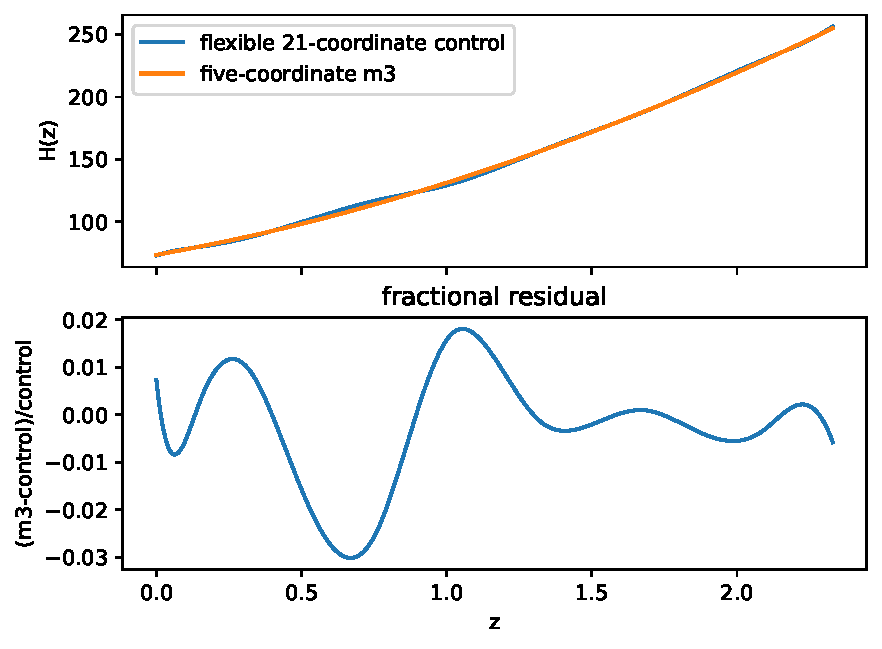
\includegraphics[width=0.9\linewidth]{figures/generated/bridge_fig2_m3}
  \caption{Five-coordinate order-3 reconstruction compared with the
  flexible 21-coordinate control. The lower panel shows
  $(H_{m=3}-H_{\rm control})/H_{\rm control}$.}
  \label{fig:reconstruction-m3}
\end{figure}

\subsection{Predictive validation and the failed continuation}

Orders above the selected $m=3$ model do not provide enough held-out improvement to overcome the predeclared parsimony rule, and still higher orders degrade predictive performance
(Table~\ref{tab:constrained-cv}). The null reconstruction is the undeformed
$\Lambda$CDM reference with zero fitted reconstruction coordinates ($K_{H}$
fixed to no deformation, $\epsilon$ not applicable) and a single
common $M$ profiled per fold-train (null contract,
\path{paper/evidence/likelihood/null_model_contract.json}).
Against this null on identical folds,
the fixed $m=3$ map improves held-out supernova prediction by
$\Delta\chi^{2}=\BridgeNullSn{}$ and improves constrained DESI
($z\le1.8$) by $\Delta\chi^{2}=\BridgeNullDesiConstr{}$ (null reconstruction
$\chi^{2}=\BridgeDesiBareConstr{}$ against
$m=3$ $\chi^{2}=\BridgeDesiMThreeConstr{}$); the order-3 reconstruction fails its $z=2.33$ Ly$\alpha$ continuation test strongly. The Ly$\alpha$ block
is then scored as an out-of-domain continuation test, where every
order shows a large continuation error (Ly$\alpha$ column of
Table~\ref{tab:constrained-cv}). The order-3 continuation
fails, and therefore the reconstruction's constrained domain ends at
$z\le1.8$; this bounds the claim rather than rescuing the model.

\subsection{Statistical interpretation of model selection}
\label{sec:prosecution}

A parametric bootstrap of the entire constrained-domain selection
pipeline under the null reconstruction (250 replicates; same null/candidate
family, data split, bounds and selection rule;
constrained
bootstrap \texttt{bootstrap.json} in paper
evidence)
gives $P(\mathrm{select} \ge m{=}3 \mid \mathrm{null}) =
\CvConstrBootProb{}$, reported exactly as obtained with no threshold
tuning. The Ly$\alpha$ continuation-failure statistic is recorded separately
and never chooses $m$. This bootstrap tests the complexity of the
selected representation, not the existence of the numerical difference
between fixed endpoint histories. Model-order selection alone is not
evidence of a discovery. The reference-sensitivity analysis is a
separate robustness check, not a significance test. The result is presented as a compact reconstruction
with demonstrated held-out behavior.

\begin{figure}[!htbp]
  \centering
  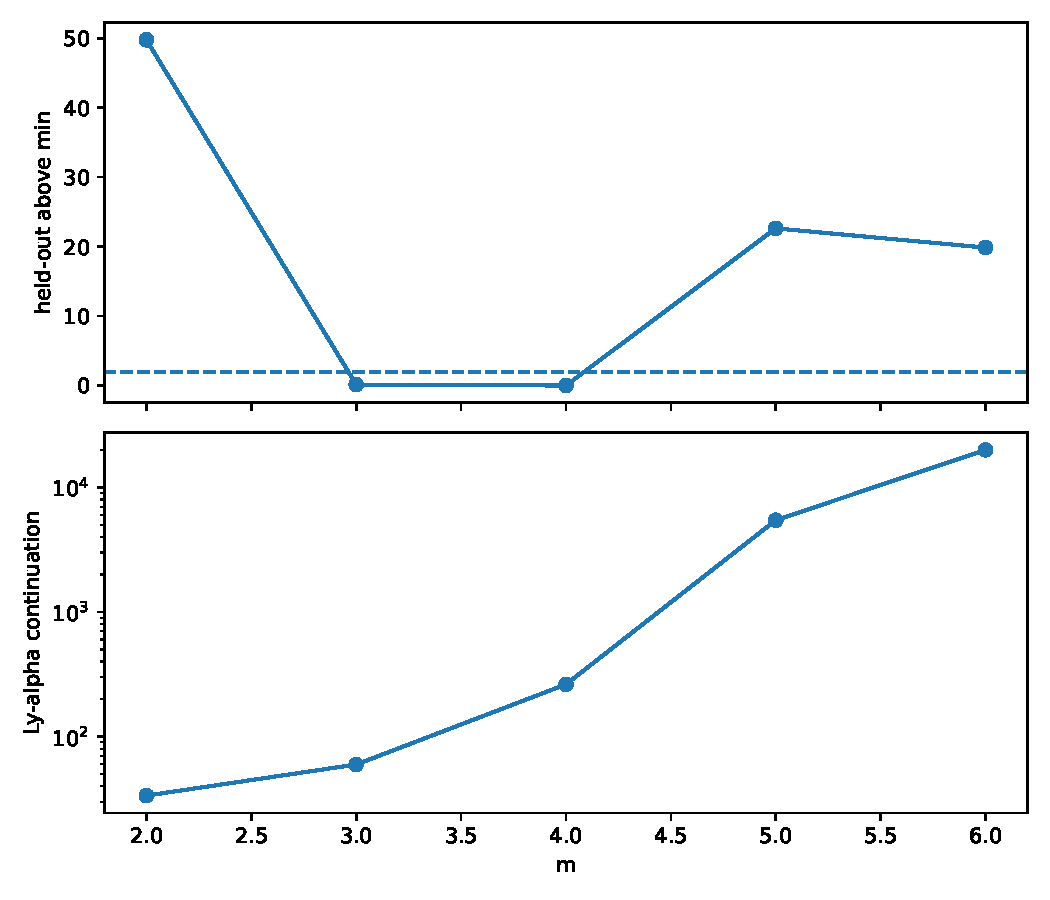
\includegraphics[width=0.9\linewidth]{figures/generated/bridge_fig3_cv}
  \caption{Constrained predictive model selection: held-out
  $\Delta\chi^{2}$ versus the constrained minimum (top; SN plus DESI
  $z\le1.8$), with the Ly$\alpha$ continuation failure on a
  logarithmic scale (bottom; not used in selection). The $m=3$/$m=4$
  near-tie is visible; the dashed line is the within-2 selection
  threshold above the minimum, and the predeclared smallest-$m$-within-2.0 rule
  selects $m=3$.}
  \label{fig:reconstruction-cv}
\end{figure}

\subsection{Reciprocity test}

The ruler/clock split is consistent with zero: $\Delta\chi^{2}
(\epsilon{=}0)=\BridgeEpsDelta{}$, with 1-sigma profile
approximately $[-0.012,+0.005]$. No nonreciprocal calibration is
detected; $\epsilon$ is not detected.

\begin{figure}[!htbp]
  \centering
  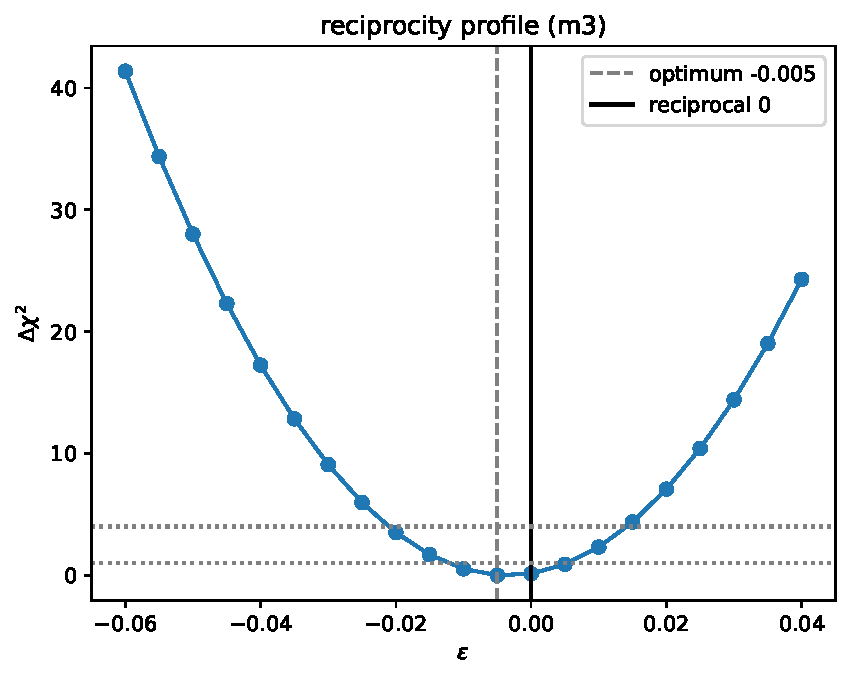
\includegraphics[width=0.9\linewidth]{figures/generated/bridge_fig4_epsilon}
  \caption{Reciprocity profile $\Delta\chi^{2}(\epsilon)$ in the
  selected $m=3$ map: optimum near $-0.005$ and zero at
  $\Delta\chi^{2}=\BridgeEpsDelta{}$, with horizontal
  $\Delta\chi^{2}=1$ and $4$ levels.}
  \label{fig:reconstruction-epsilon}
\end{figure}

\subsection{Why increased flexibility is rejected}
\label{sec:diagnostic-alternatives}

The analysis actively rejected better-looking training solutions. The
roughness family reaches $\chi^{2}=1453.34$ but its leading shape
coefficient sits exactly at the imposed bound ($c_{1}=+0.5$) with
the local descent gradient pointing outward, so its optimum depends
on the box: it is boundary-limited and retained as a supporting
basis only. The Legendre $m=6$ map reaches good training
$\chi^{2}=1455.19$ with an interior optimum but fails the held-out
Lyman-alpha continuation test (Table~\ref{tab:constrained-cv});
it is therefore not promoted.
Both are retained as fixed diagnostic alternatives in
evidence.

% Ch 5. Reference sensitivity.
\section{Reference sensitivity}
\label{sec:reference-sensitivity}

The reconstruction above is
measured against one particular CMB-compatible history~C1. This
section repeats the comparison against a second, separately implemented
CMB-compatible history~C2 and shows the deformation is
shared. All headline metrics resolve from versioned publication evidence JSON through
registry macros, never handwritten.

\subsection{Endpoint invariance}

Define the logarithmic difference fields on the common grid
(Section~\ref{sec:endpoint-repr}):
\begin{equation}
  \Delta_{1}(z)=\ln H_{R}(z)-\ln H_{C1}(z),
  \label{eq:delta1}
\end{equation}
\begin{equation}
  \Delta_{2}(z)=\ln H_{R}(z)-\ln H_{C2}(z),
  \label{eq:delta2}
\end{equation}
\begin{equation}
  \Delta_{C}(z)=\ln H_{C1}(z)-\ln H_{C2}(z),
  \label{eq:deltaC}
\end{equation}
with the common and disagreement combinations
\begin{equation}
  \Delta_{\rm common}(z) = \frac{\Delta_{1}(z)+\Delta_{2}(z)}{2},
  \label{eq:common}
\end{equation}
\begin{equation}
  \Delta_{\rm disagreement}(z) = \frac{\Delta_{1}(z)-\Delta_{2}(z)}{2}.
  \label{eq:disagreement}
\end{equation}
The quoted common-mode fraction is
\begin{equation}
  f_{\rm common}
  =
  1-
  [
  \frac{\mathrm{RMS}(\Delta_{\rm disagreement})}
       {\mathrm{RMS}(\Delta_{\rm common})}
  ]^2,
  \label{eq:fcommon}
\end{equation}
evaluated per redshift interval on the constrained domain.
Changing the CMB reference history from C1 to C2 does not change the
hypothesis: the same compact map must describe both separations.

\subsection{Common-mode decomposition}

On the constrained domain ($z\le1.8$), the R–C1 and R–C2 difference fields lie
substantially on top of one another. The common-mode fraction
exceeds~\GeometryCommonFractionMin{} in every redshift interval, and
the two-vector singular decomposition is dominated by a single
shared direction (dominance ratio~\GeometrySvdDominance{}). The two
fields peak at the same location, near
$z\approx\GeometryPeakZ{}$, while across the constrained bins the
C1–C2 RMS difference is approximately \ReferenceSensitivityRatioMinPct{}\% to \ReferenceSensitivityRatioMaxPct{}\% of the corresponding RMS difference between R and either Planck reference.

\subsection{Peak location and data support}
\label{sec:peak-support}

The fitted endpoint difference reaches its maximum near
$z\simeq0.65$. The peak does not coincide with the maximum Pantheon+ number density, supernova inverse-variance weight, or a simple DESI BAO information-density maximum. The order-3 reconstruction captures the broad low/intermediate-redshift structure but reaches its own maximum near $z\simeq0.39$.

\subsection{Cross-reference transfer}

The fixed order-3 basis transfers across references: shape amplitudes
refit independently agree, and parameters learned on one CMB reference
predict the other separation with residual degradation fraction
\GeometryTransferDegradation{} ($\le 6.8\%$ cross-reference). One
dominant shared direction carries the deformation; the residual
endpoint-specific component is small.

\subsection{Statistical status of the reference-sensitivity test}
\label{sec:reference-sensitivity-stats}

The order-selection bootstrap tests model complexity; it does not
test reference-construction similarity. The reference-sensitivity metrics quantify robustness of fixed
best-fit histories: how much the measured R-versus-CMB separation moves
when the CMB reference construction changes. C1 and C2 are not
statistically independent (both use Planck information;
Section~\ref{sec:endpoint-c2}), and the two difference fields share
the same R endpoint ($\Delta_{1}=R-C_{1}$,
$\Delta_{2}=R-C_{2}$), so their similarity is mathematically
correlated. Endpoint posterior uncertainty was not propagated.
Therefore no frequentist p-value is assigned to the cosine or
common-mode statistic. The reference-sensitivity test shows a
shared low-dimensional deformation across the tested constructions.

\subsection{Constrained domain and Ly\texorpdfstring{$\alpha$}{alpha} continuation}

All reference-sensitivity metrics above are quoted on the constrained
domain $z\le1.8$, covering every non-Ly$\alpha$ DESI block. The
Ly$\alpha$ anchor at $z=2.33$ is a continuation test of the
reconstruction law, not a measurement of the low-redshift
deformation: flexible extrapolators generically fail there, under
the null as on the data (Ly$\alpha$ continuation-failure fraction
\CvConstrLyaProb{} in the matched constrained-domain bootstrap,
recorded separately and never used in selection).

\subsection{Comparison with the fit-improvement attribution}

The deformation RMS (peak bin $0.4<z<0.8$) and the
fit-improvement attribution (peak bin $0<z<0.4$) both concentrate
below $z\sim0.8$, though their peak bins differ; high-redshift behavior
is unconstrained in both. Thus the order-3 representation is accurate as a broad-shape reconstruction but is not an exact peak-localization model. The reference-sensitivity check therefore supports, rather
than replaces, the compact reconstruction: the same
five-coordinate map describes a deformation that is
reference-insensitive within the two tested Planck-compatible constructions.

\begin{figure}[!htbp]
  \centering
  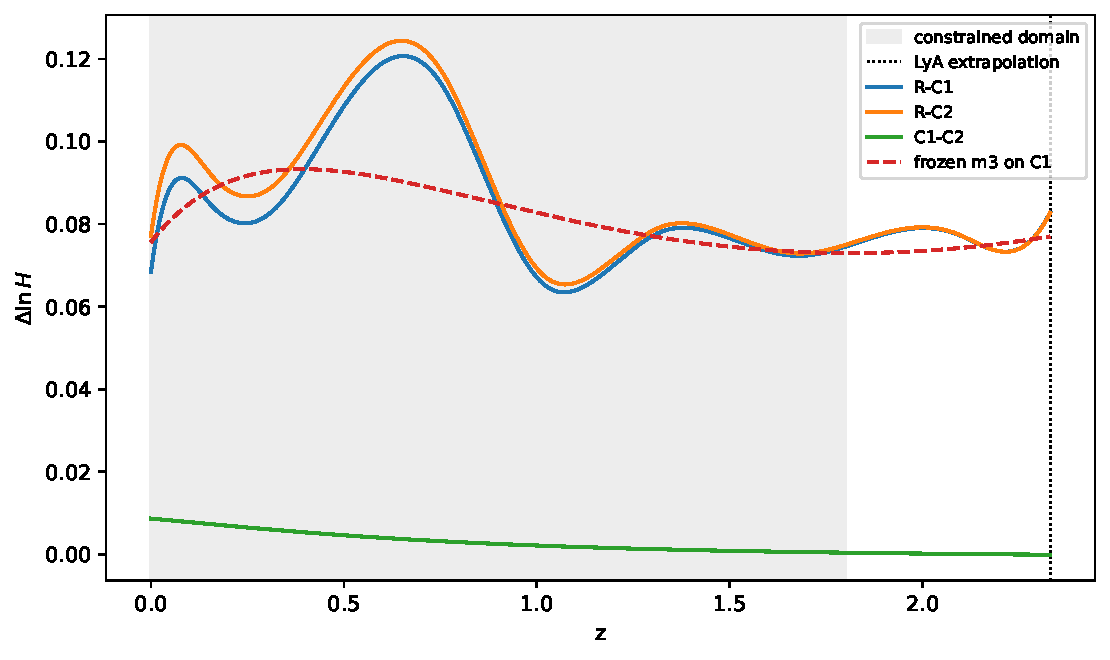
\includegraphics[width=0.9\linewidth]{figures/generated/bridge_fig5_triangulation}
  \caption{Reference-sensitivity overlay: the R–C1 and R–C2 difference fields
  lie on top of one another across the constrained domain (R–C1 and R–C2 nearly coincide; the C1–C2 difference is much smaller), and the
  fixed order-3 reconstruction captures the broad low/intermediate-redshift
  trend but not the exact peak near $z\simeq0.65$. Shading marks the
  constrained domain; the dotted line marks the Ly$\alpha$
  extrapolation test.}
  \label{fig:reference-sensitivity}
\end{figure}

% Ch 6. Results (nests endpoint-construction detail subsections).
\section{Results}
\label{sec:results}

This section states the paper's empirical results in one place.
Construction details are in
Sections~\ref{sec:data-endpoints}--\ref{sec:robustness}.
Headline numerical results are generated from or hash-bound to frozen evidence.

\subsection{Headline branch separation}

The phenomenological low-redshift distance-sector endpoint~R
($H_{0}=\DistanceHZero$\kmsMpc{}; not presented as a complete cosmological model) differs substantially from both
Planck-compatible references C1 ($H_{0}=\CmbOneHZero$\kmsMpc{}) and
C2 ($H_{0}=\CmbTwoHZero$\kmsMpc{}, secondary sensitivity reference) across the constrained domain
$z\le1.8$.
The two R--CMB difference fields
$\Delta_{1}$ and $\Delta_{2}$ (defined in Section~\ref{sec:endpoint-repr})
share one dominant common
mode (common-mode fraction $\ge\GeometryCommonFractionMin{}$ per
interval), while the CMB--CMB difference
$\Delta_{C}$ is much smaller throughout: across the constrained bins,
the C1--C2 RMS difference is about 1--8\% of the R--CMB difference
(RMS ratios \GeometryCmbRatioLow{} and
\GeometryCmbRatioHigh{} on the constrained and high intervals).

\subsection{Compact reconstruction}

A five-coordinate order-3 (m3) map gives a compact empirical
description of the constrained-domain ($z\le1.8$) branch difference with local projected Jacobian rank~5
of~5 fitted coordinates ($\chi^{2}=\BridgeChiTwo{}$, only \BridgeDeltaCtrl{} above the
21-coordinate control; $\mathrm{AIC}\approx\BridgeAIC{}$ against
$\approx\BridgeAICCtrl{}$ for the control, reported descriptively as
parsimony rather than evidence). Selection is
predictive (held-out supernova and DESI $z\le1.8$ folds,
Section~\ref{sec:bridge}) and carries no significance of
its own: the matched constrained-domain null bootstrap tests representation complexity, not
existence of the endpoint separation (null bootstrap
$P(\mathrm{select}\ge m3)=\CvConstrBootProb{}$).
Zero ruler-clock split is allowed
($\Delta\chi^{2}(\epsilon{=}0)=\BridgeEpsDelta{}$).
The fitted difference reaches its largest
amplitude near $z\approx\GeometryPeakZ{}$; because this region also
carries substantial observational leverage, we do not interpret the
peak redshift as a fundamental physical scale
(Section~\ref{sec:peak-support}).

\subsection{Reference-branch robustness}

The frozen m3 basis transfers across the two Planck references with small
residual degradation (fraction \GeometryTransferDegradation{}):
parameters learned on
one reference construction predict the other separation. The two R--CMB fields
share one dominant direction
(cosine~\GeometryCosineSimilarity{}, principal angle
\GeometryPrincipalAngle$^{\circ}$). This reference-sensitivity
check shows the deformation is insensitive to the tested
CMB-reference construction; it does not assign a frequentist
p-value to the similarity (Section~\ref{sec:robustness-stats}).
Neither branch fits everything and no tension resolution is claimed.
High-redshift continuation through the
Lyman-alpha anchor remains unvalidated.

\FloatBarrier
\section{Discussion}
\label{sec:discussion}

\subsection{What appears robust}
\label{sec:robust}

Within the tested reconstructions over $z\le1.8$, six features recur. First, a
common R--CMB deformation: the two R--CMB difference fields lie on
top of one another (common-mode fraction
$\ge\GeometryCommonFractionMin{}$ per interval). Second, a peak near
$z\approx\GeometryPeakZ{}$ (largest amplitude; not a fundamental
scale). Third, low/intermediate-$z$
concentration: both the deformation RMS (peak bin $0.4<z<0.8$)
and the
fit-improvement attribution (peak bin $0<z<0.4$) concentrate below
$z\sim0.8$, though their peak bins differ. Fourth, one
dominant shared direction (cosine~\GeometryCosineSimilarity{},
principal angle \GeometryPrincipalAngle$^{\circ}$, SVD dominance
\GeometrySvdDominance{}). Fifth, a compact representation: five
coordinates suffice
($\chi^{2}=\BridgeChiTwo{}$, local projected Jacobian rank~5 of~5
fitted coordinates,
$\mathrm{AIC}\approx\BridgeAIC{}$ against
$\approx\BridgeAICCtrl{}$ descriptively). Sixth, reference
insensitivity across C1/C2:
cross-branch transfer degrades by fraction
\GeometryTransferDegradation{} or less while the CMB--CMB
difference stays much smaller (about 1--8\% of the R--CMB difference
across the constrained bins).

\subsection{What is not established}
\label{sec:not-established}

No physical origin is established. No fundamental metric
modification and no modified gravity are
demonstrated. R is a phenomenological low-redshift endpoint, not
presented as a complete cosmological model: it describes what the fitted low-redshift distance
sector prefers, with no claimed recombination, BBN, or perturbation
completion. No tension resolution is claimed: neither branch fits
everything. No statistical significance is claimed for the
representation complexity: the matched constrained-domain null
bootstrap gives
$P(\mathrm{select}\ge m3)=\CvConstrBootProb{}$, so order
selection alone is not evidence. No high-redshift continuation law
is validated: the Ly$\alpha$ anchor is an extrapolation test that
flexible maps generically fail.

\subsection{Possible physical interpretations}
\label{sec:interpretations}

We list categories, not endorsements. A first category is evolving
late-time background dynamics (dark-energy-like histories reproducing the
same $H(z)$ deformation). A second is early-universe and ruler physics
(recombination or drag-epoch effects shifting the acoustic scale, or
combinations of early and late effects). A third is modified
gravity and modified propagation (distance-duality or
luminosity-distance effects mimicking expansion structure). A fourth
is conventional systematics or calibration effects in one or more of
the distance, BAO, or CMB sectors.

\subsection{What would discriminate interpretations}
\label{sec:discriminate}

Untouched sectors would discriminate where background geometry
cannot. Independent tests include cosmic chronometers, redshift-space
distortions, weak and CMB lensing, time-delay distances, and standard
sirens. No fitting in those sectors is
performed in this paper.

\section{Limitations}
\label{sec:limitations}

All reported values are best fits; no posterior intervals are claimed. Endpoint posterior uncertainty is not propagated into the difference fields. C1 and C2 are not statistically independent constructions: both use Planck information. R carries $r_{d}=135.39$~Mpc while the C1/C2 references use recomputed CAMB rulers near $147.1$~Mpc (Table~\ref{tab:calibration}). The constrained reconstruction domain is $z\le1.8$; the order-3 continuation fails at the $z=2.33$ Ly$\alpha$ anchor. The calibrator result covers the declared contract only ($\Delta\mu_{\mathrm{cal}} = 0$, a qualitative assumption, not quantitatively established).

\begin{table}[!htbp]
  \centering
  \caption{Limitations and current status.}
  \label{tab:limitations}
  \begin{tabular}{ll}
    \toprule
    Issue & Current status \\
    \midrule
    Endpoint posterior uncertainty & Not propagated \\
    C1/C2 statistical independence & Shared Planck information \\
    Order-selection bootstrap & $P = 0.216$ \\
    Constrained reconstruction range & $z \le 1.8$ \\
    Ly$\alpha$ continuation test & Fails at $z = 2.33$ \\
    \bottomrule
  \end{tabular}
\end{table}

The distance-sector endpoint and the Planck-compatible
references prefer quantitatively different expansion histories
($H_{0}$ \DistanceHZero{} vs \CmbOneHZero{}, with endpoint-specific
acoustic rulers per Table~\ref{tab:calibration}).

\subsection{Relation to neighbouring approaches}
\label{sec:literature}

DESI DR2 BAO remain compatible with flat $\Lambda$CDM in isolation,
while combinations with CMB and supernovae can favor evolving dark
energy of the $w_{0}w_{a}$ form~\citep{DESIDR2,
Chevallier2001,Linder2003}. Our reconstruction is not a dark-energy equation of
state: it is a reconstruction of the
required observational transformation between two calibrated
histories, with dimensionality selected through held-out data rather
than by allowing enough function freedom to improve the joint fit.
That selection discipline is also what separates this work from
unconstrained Gaussian-process or smoothing reconstructions of the
expansion history~\cite{Shafieloo2006} and from generic
cosmography~\cite{Cattoen2007}, which do not penalize flexibility by
prediction. Early-dark-energy solutions modify the pre-recombination
universe and its perturbations; the reconstruction assumes no recombination
change and carries no perturbation sector. For the broader solution
landscape we refer to the community review~\cite{DiValentino2021}.
This work does not introduce another
equation-of-state fit. It compares separately calibrated histories
and asks whether their difference is compact and
reference-insensitive within the two tested Planck-compatible
constructions. This decomposition is complementary to the scale-vs-shape
obstruction argument \citep{Zhou2026}: uniform sound-horizon rescaling
changes scale but cannot remove the BAO--SN shape disagreement, and our
R endpoint contains both a large ruler shift ($\sim8\%$) and a
redshift-dependent shape difference.

\section{Conclusion}
\label{sec:conclusion}

Over the constrained domain $z\le1.8$, the two Planck-compatible
references are much closer to each other than
either is to~R: across the constrained bins the C1--C2 RMS difference
is about 1--8\% of either R--CMB difference. Changing between these two Planck-compatible references
changes the inferred difference only slightly (reference sensitivity,
not independent confirmation).

The two R--CMB difference fields over $z\le1.8$ are nearly identical:
they share one dominant direction
(cosine~\GeometryCosineSimilarity{}, principal angle
\GeometryPrincipalAngle$^{\circ}$) with cross-branch transfer
degradation fraction \GeometryTransferDegradation{} or less, reaching
largest amplitude near $z\sim\GeometryPeakZ{}$ without that redshift
being claimed as a fundamental physical scale.

A five-coordinate $m3$ basis provides a compact empirical
description over $z\le1.8$ ($\chi^{2}=\BridgeChiTwo{}$, local
projected Jacobian rank~5 of~5 fitted coordinates),
but its selection is not itself statistically significant under the
null bootstrap
($P(\mathrm{select}\ge m3)=\CvConstrBootProb{}$), which tests the complexity of
the representation rather than the existence of the numerical
difference between frozen endpoint histories. Continuation to
Ly$\alpha$ at $z=2.33$ fails for the compact extrapolator, bounding
the validated domain to $z\le1.8$.

The physical origin remains open: no dynamics, no metric theory,
and no tension resolution are established here. R is a
phenomenological low-redshift endpoint, not presented as a complete
cosmological model.

The resulting target is the low-redshift distance-sector behavior
represented by R over $z\le1.8$, together with the requirement that
any physical completion preserve the observed CMB acoustic structure;
R itself is not asserted to be such a completion.


\clearpage\appendix
% Publication appendices only.
\section{Likelihood details and calibration contract}
\label{app:likelihood}

The joint likelihood sums DESI DR2 BAO terms with published
covariances, the compressed CMB prior used during endpoint discovery,
and the Pantheon+SH0ES joint term. No external $H_{0}$ prior enters
the likelihood.

Pantheon+SH0ES is one 1657-row covariance likelihood with one common
profiled $M$. With $r_{0}=m_{B}^{\mathrm{corr}}-\mu_{\mathrm{no}\,M}$,
\begin{equation}
  \hat{M} = \frac{\mathbf{1}^{T}C^{-1}r_{0}}
                 {\mathbf{1}^{T}C^{-1}\mathbf{1}},
  \qquad
  \chi^{2}_{\mathrm{joint}}
    = (r_{0}-\hat{M}\mathbf{1})^{T}C^{-1}(r_{0}-\hat{M}\mathbf{1}),
\end{equation}
where $C$ is the full $1657\times1657$ covariance. Ladder and
non-ladder blocks are diagnostics: each uses its marginal covariance
with an independent $M$, so
$\chi^{2}_{\mathrm{ladder}}+\chi^{2}_{\mathrm{non\text{-}ladder}}
\neq \chi^{2}_{\mathrm{joint}}$.

Calibrator rows use $\mu_{\mathrm{cal}}=\mathrm{CEPH\_DIST}$.
Under the adopted calibration contract, no additional theory-side
correction is applied to local calibrator distance moduli:
$\Delta\mu_{\mathrm{cal}}=0$; this covers the declared contract only
and is a qualitative assumption, not quantitatively established.
Hubble-flow rows use $z_{\mathrm{HD}}$
for $D_{M}$ and the $z_{\mathrm{HD}}$/$z_{\mathrm{HEL}}$ prefactor
$D_{L}=(1+z_{\mathrm{HEL}})D_{M}(z_{\mathrm{HD}})$, which assumes massless
photons, null geodesics, and photon-number conservation
\citep{Etherington1933}.

The endpoint-discovery CMB block is the compressed set
$(R,\ell_{A},\omega_{b}h^{2})$ with numerical values from
\citep{Chen2019}, validated there against conventional late-time
models only. Endpoint R was originally selected using the Chen et al. compressed Planck distance prior. Because those priors were validated for conventional late-time models, they are not used here as evidence that R's nonstandard ruler is physically viable. The C1/C2 reference constructions are calibrated directly to the
full Planck spectra (Section~\ref{sec:data}).

\subsection{Calibration contract}
No telescope or catalog data were rescaled. All changes are in the
forward model, not the data: observed redshifts, magnitudes,
covariances, masks, and Cepheid distances are untouched.

DESI path: $z_{\mathrm{obs}}\to z_{\mathrm{bg}}\to
D_{M},D_{H},D_{V}\to D/r_{d}$ with each endpoint's own ruler from
Table~\ref{tab:calibration}; observed
$D/r_{d}$ rows and published covariances are unchanged.
Pantheon+SH0ES path: 1657 selected rows including 77 calibrators;
$z_{\mathrm{HD}}$ for cosmological distance, $z_{\mathrm{HEL}}$ in
the luminosity prefactor, CEPH\_DIST for calibrator $\mu$; one
common profiled $M$ with full $1657\times1657$ covariance in the fit;
source-defined ladder split is diagnostic-only with independent $M$
terms and is non-additive under the joint cross-covariance.

\begin{figure}[!htbp]
\centering
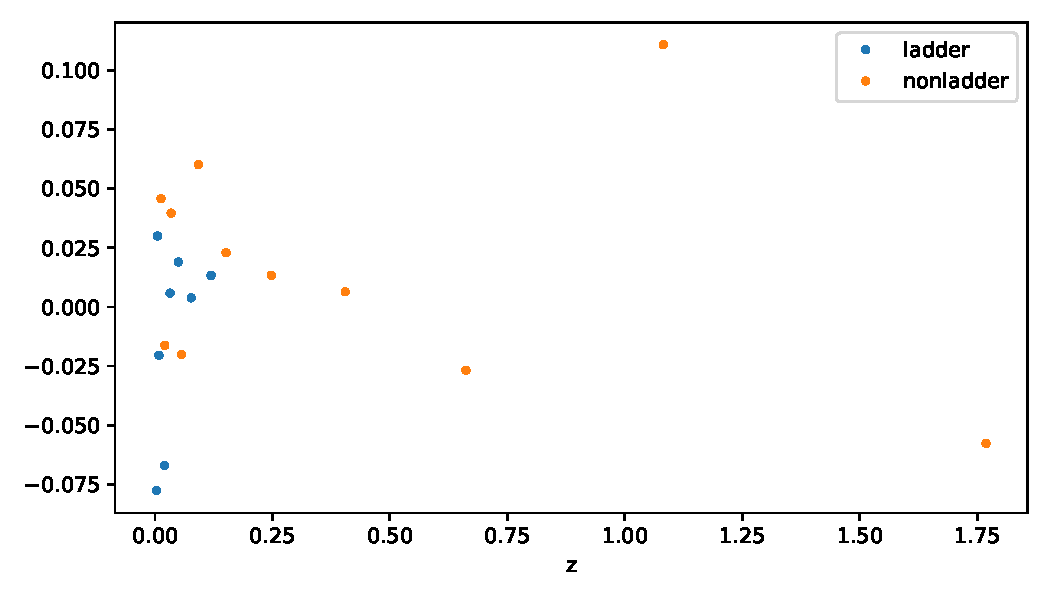
\includegraphics[width=0.9\linewidth]{figures/generated/figure_A_sn_subset_diagnostics.pdf}
\caption{Appendix-only subset-profiled supernova diagnostics:
source-defined ladder diagnostic, independently profiled $M$ (left) and
complementary non-ladder diagnostic, independently profiled $M$ (right).
Non-additive; never used in the joint fit.}
\label{fig:sn-subset}
\end{figure}

\section{Reproducibility}
\label{app:repro}

The driver \path{scripts/paper/build_expansion_history_paper.py}
replays the versioned publication evidence, rebuilds the results registry,
regenerates all figures and tables with source-hash binding, validates
claims in release mode, compiles the manuscript with pdflatex and
bibtex, and builds and checks the arXiv bundle. The bundle
\path{paper/dist/arxiv_submission/} is flat and self-contained,
excluding run directories, source code, tests, credentials, logs, and
caches. Random seeds, code hashes, and data hashes are recorded in the
versioned publication evidence manifests.

Numerical stack. All array arithmetic uses NumPy \citep{Harris2020} and
all optimization and quadrature use SciPy \citep{Virtanen2020};
versions are pinned in the versioned publication evidence manifests.
Fixed endpoint artifacts and their hashes are listed in
\path{paper/evidence_manifest.yaml}; regeneration fails on hash
mismatch, so the published numbers reproduce exactly from the
archived evidence. Every build step reads only files inside this
public repository; no step reaches outside it.

\subsection{Code and data availability}
The paper source, derived publication evidence, reproducibility scripts, and interactive visualization are available at \url{https://github.com/jenholm/physics_models/tree/main/redshift-dependent-expansion}. Public evidence records include the R endpoint history (\url{https://github.com/jenholm/physics_models/blob/main/redshift-dependent-expansion/paper/evidence/endpoints/endpoint_redshift.json}), the C1 reference (\url{https://github.com/jenholm/physics_models/blob/main/redshift-dependent-expansion/paper/evidence/endpoints/endpoint_cmb_1.json}), the C2 reference (\url{https://github.com/jenholm/physics_models/blob/main/redshift-dependent-expansion/paper/evidence/endpoints/endpoint_cmb_2.json}), the constrained-domain definition (\url{https://github.com/jenholm/physics_models/blob/main/redshift-dependent-expansion/paper/evidence/endpoints/domain_split.json}), the reference-sensitivity metrics (\url{https://github.com/jenholm/physics_models/blob/main/redshift-dependent-expansion/paper/evidence/reference_sensitivity/scale_comparison.json} and \url{https://github.com/jenholm/physics_models/blob/main/redshift-dependent-expansion/paper/evidence/reference_sensitivity/agreement_metrics.json}), and the model-selection and bootstrap evidence (\url{https://github.com/jenholm/physics_models/blob/main/redshift-dependent-expansion/paper/evidence/model_selection/constrained_cv.json} and \url{https://github.com/jenholm/physics_models/blob/main/redshift-dependent-expansion/paper/evidence/model_selection/bootstrap.json}).


\bibliographystyle{unsrtnat}
\clearpage\bibliography{references}

\end{document}
